% House style for paper-ready plots in pgfplots/TikZ, with two examples:
% a line plot (method vs baselines) and a radar chart for multi-metric
% comparisons. Copy the preamble block into the paper; replace the inline
% tables with `\addplot table [col sep=comma] {data.csv};`.
\documentclass[border=2pt]{standalone}
\usepackage{pgfplots}
\pgfplotsset{compat=1.18}

% --- house style (preamble) ---------------------------------------------
\definecolor{method}{HTML}{3F21B6}     % primary method
\definecolor{secondary}{HTML}{8C7AD3}  % secondary method of ours
\definecolor{baseline}{HTML}{BDBDBD}   % every baseline or comparison
\pgfplotsset{
  house/.style={
    width=6.5cm, height=4.4cm,
    axis lines=left, axis line style={-}, tick align=outside,
    tick label style={font=\scriptsize}, label style={font=\footnotesize},
    legend style={draw=none, fill=none, font=\scriptsize},
    legend cell align=left,
    every axis plot/.append style={line width=0.9pt, mark size=1.2pt},
  },
  method/.style={color=method, mark=*},
  secondary/.style={color=secondary, mark=triangle*},
  baseline/.style={color=baseline, mark=square*, densely dashed},
}

% Radar chart: \radar{<style>}{<values in [0,1], one per axis, outward = better>}
% Requires \radarN (number of axes) and \radarR (radius) to be set.
\newcommand{\radar}[2]{%
  \foreach \v [count=\i from 0] in {#2}
    \coordinate (r\i) at ({90-360/\radarN*\i}:{\v*\radarR});
  \pgfmathtruncatemacro{\radarlast}{\radarN-1}
  \draw[#1] (r0) \foreach \i in {1,...,\radarlast} { -- (r\i) } -- cycle;
}
% ------------------------------------------------------------------------

\begin{document}

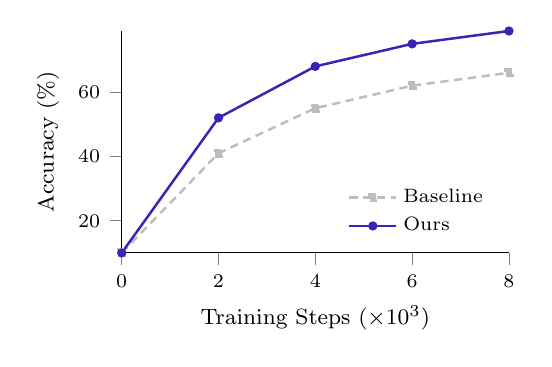
\begin{tikzpicture}
\begin{axis}[house, xlabel={Training Steps ($\times 10^3$)}, ylabel={Accuracy (\%)},
             legend pos=south east]
  \addplot[baseline] table [row sep=\\] {x y \\ 0 10 \\ 2 41 \\ 4 55 \\ 6 62 \\ 8 66 \\};
  \addlegendentry{Baseline}
  \addplot[method] table [row sep=\\] {x y \\ 0 10 \\ 2 52 \\ 4 68 \\ 6 75 \\ 8 79 \\};
  \addlegendentry{Ours}
\end{axis}
\end{tikzpicture}
\qquad
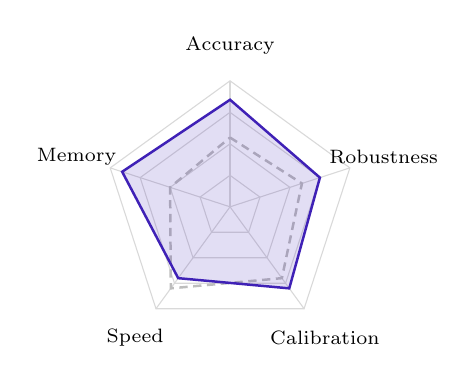
\begin{tikzpicture}[font=\scriptsize]
  \def\radarN{5}\def\radarR{1.6}
  % polygonal grid and spokes
  \foreach \g in {0.25,0.5,0.75,1} { \radar{black!15}{\g,\g,\g,\g,\g} }
  \foreach \lab [count=\i from 0] in {Accuracy,Robustness,Calibration,Speed,Memory} {
    \draw[black!15] (0,0) -- ({90-360/\radarN*\i}:\radarR);
    \node at ({90-360/\radarN*\i}:{\radarR+0.45}) {\lab};
  }
  \radar{draw=baseline, densely dashed, line width=0.9pt}{0.55,0.6,0.7,0.8,0.5}
  \radar{draw=method, line width=0.9pt, fill=method, fill opacity=0.15}{0.85,0.75,0.8,0.7,0.9}
\end{tikzpicture}

\end{document}
